\section[第9章\q 拿铁因子]{第9章\\ 拿铁因子}
\label{sec:ch9}

快到海伦娜咖啡厅时，亨利正步出大门。

“喔，”他说，“很高兴不期而遇。”

“我有个问题想请教，”柔伊说话时，依然喘着气。

“请说。”亨利回答。他回头看了看自己身后，又看了看柔伊身后，对她说：“一起去咖啡厅坐一坐？”

柔伊想说好，跟他回海伦娜。不想，他迈着轻快的步子，穿过了街道。她跟上去。到街角之后，他停住了，打开了第一家店的门。

是一家星巴克。

柔伊犹豫了一下，看着他，好像在说：你是认真得吗？

“请进。”亨利笑着说。

他们走了进去，来到点餐柜台前。

\subsection{你在帮谁累积财富？自己还是别人？}

“特浓拿铁，谢谢。”柔伊说。然后，又加了一句：“可以做低咖啡因的吗？一半咖啡因？”

“一杯热茶，”亨利说。“英式早餐那种。”

说完，亨利付了两杯饮料的钱。尽管柔伊要自己付钱，但是亨利很坚持，他就是一位老派绅士。柔伊笑着接受了。他们走去咖啡厅后方的小桌子。

“我也说不上来，”柔伊说，“和你坐在星巴克，感觉非常奇怪。好像背叛你家咖啡厅的感觉。”

亨利笑着说：“有吗？”

“有啊！”柔伊啜了一口拿铁，“我猜，你是来了解敌情的吧！”她用装咖啡的纸杯碰了一下亨利装着热茶的纸杯，“耶！我们现在成功卧底了。”

亨利脸上的笑颇为神秘。他拉着茶包，往热水里浸了两、三回。

“我得坦白一下。”柔伊开口说，“在昨天，知道你就是咖啡厅老板之前，我一直想问你‘一位咖啡师，如何知道累积财富的秘密？’”

亨利把茶包里挤干放到一旁，正色看着柔伊：“你的意思是，如果‘先付钱给自己’一招有效，怎么会有个像我这样70岁的老人，还在打工维生？”

柔伊的脸涨红了，低着头说：“我，也不是那个意思……”她又看了看亨利，带着歉意的笑着：“好吧，多少也有点那个意思。”

亨利露齿而笑，然后吹着气，让热茶冷一点。“我可以说一下我的背景，没问题的。我草创海伦娜咖啡厅是在三十多年前了，附近同行朋友很多。后来，现在他们都走了……”

“喔，对不起。”柔伊说，但是亨利却也只是笑一笑。

“不是，你误会了，他们不是挂了。他们只是离开了，或者转做其他行业。你知道我为什么还能留在这里吗？为什么我的咖啡厅还能继续营业吗？”

“因为咖啡味道好？”柔伊说，“当然，不只如此。还有气氛好。”亨利继续不置可否的笑着。“还有一群你的死忠粉丝？”

亨利大笑起来：“谢谢你这么说，但其实还有其他。我能继续待在这里，是因为我买下了这栋大楼。”

“你买下了这栋大楼？”柔伊重复说。

“以及隔壁一栋。”亨利说，“还有同一条街上另外几处房子。”

这下，柔伊惊讶得说不出话来。她以为的“古怪咖啡师”就有这等来头，她得把原本的想像图象好好编辑一下。

“基本来说，人可以分成两种。每个人每天都花钱，花钱也是累积财富。每个人都在累积财富。\textbf{差别在于，为谁累积？}”

“你提到了在外头租屋。租屋时，你就把生活的主动权交了出去。如果拥有住屋，那就拥有了部分的生活自主权。拿我的例子来说，做事业的自主权是握在自己手上。

“再拿星巴克来说。他们刚开始的时候，每个人都认为开什么玩笑，卖昂贵咖啡也能成为一门生意？就算可以，也不可能长久。但现在他们长久了，而且还卖到全世界去。所以，其他咖啡店倒啦！我的同行们开始不安焦虑，他们想要与星巴克对抗。他们去游说政客，想要联手反抗。”

亨利说完，停顿了一下。柔伊知道重点要来了。“你呢？”她催促。

亨利笑着说：“我买了他们的股票。”

柔伊放下咖啡，瞪着亨利：“等一下，你买了星巴克的股票？”

“是的，我买了他们的股票。就在别人，要不然买他们的咖啡，要不然抵制他们的咖啡时，我买了他们的股票。你也可以说，这是化敌为友。”

“星巴克的咖啡。”柔伊重复着。亨利身体前趋，用食指点着桌面，加强重点了说道：“如果1992年星巴克股票上市的时候，买下1,000美元的股票，你知道现在市值多少吗？”

“完全没概念。”柔伊说。

“将近25万。”

“哇，”柔伊说。“看来你的敌人还为你赚了不少。”

亨利笑了起来。“你可以这么看，我也可以从另外的角度来看。每一个进来星巴克的人，点了一杯咖啡之后，两件事就发生了：他们对这个事业投入很少的金额。一杯咖啡的钱。而因为我买了股票，也就是小股东，因此也就小赚了一点点。”

柔伊想到了亨利刚刚说的“两种人”。

亨利点头说：“没错。事业的投入者和事业的拥有者。最棒的一点是，你可以在任何时间点，选择你要做哪种人。

“当你决定先付钱给自己时，不管是10美元，或是25美元，不管是买一个自住宅，或是商业用宅，或者投资某家公司的股票，或者以某种方式投资于自己的未来，你就成为自己生活的主人。”

“许多人把自己的人生出让给别人。先付钱给自己，并养成习惯，持之以恒，积年累月之后，你就会拥有自己的人生。”

“拿你的例子来说，就是拥有了自己的事业。”柔伊说。

亨利点头。“我买下那栋房子时，我不单投资了自己，更投资了邻里。这些年下来，价值涨至100万美元了。现在重点来了，我怎么有资金买下商业大楼？我可以向你保证，我没中乐透，也没写出一首畅销歌，或者在自家后院挖到财宝。”

“也没有谋杀你有钱的姨妈？”

亨利笑着说：“没有富裕的亲戚可以攀附。真的，柔伊，是我白手创建起来的，就是先付钱给自己。”

柔伊露出在思考的样子，亨利知道她脑中依然有疑问。

“把你的问题说出来，我们来讨论一下吧！”他说。

“好的。”柔伊犹豫了一下说。“我重新看了表格。那个每天存25美元的，我猜想应该是存到银行的，40年后，就有300万了？可是这25美元是从哪里来的？”

“喔！这个问题。”亨利又朝茶杯上吹了吹。

“你又说，收入高不是解决之道。”柔伊接着说，“接着你又说，该把收入的10％存起来。或者准确来说，是1个小时的收入，其实若以8小时来算，就是12％的了。这些理论上都对。问题是，我就已经入不敷出了。”

亨利点头。“你的疑问没错，那就是为什么要说拿铁因子。”

\subsection{拿铁因子，是那些非必要的消费习惯}

亨利伸手到口袋里，掏出一张5美元的纸钞，放在两人中间的桌面上。“记得这个吧？”

“1天5美元。”她说。“复利的魔力。”

“非常正确。”亨利说。“现在我们来说一说你喝的咖啡。”

柔伊看着她咖啡因减半的特浓拿铁，然后又看着亨利：“好的，来说说我的咖啡吧！”

“那杯拿铁，多少钱？4美元？”亨利问。

“4.5美元。”柔伊说。

“好，现在我们就来看看这个无足轻重的小钱。让我们看看加入复利这个因素后，会发生什么事。我们先把‘无足轻重’的4.5美元加到你的照片帐户里。1周5天，我们用1年来看。先不考虑利息，我们来看一看，”他低头计算着。“哇，就有1,200美元了。”他看着柔伊，“你还记得那张照片的标价吗？”

柔伊记得，刚好就是1,200元。

柔伊看了看拿铁，又看了看亨利。再开口说话时，语带激动。“你是说我1年喝咖啡的钱够买那张照片？”

亨利喝了一口茶。不说话。

“哇，这杯拿铁好强大啊！”

亨利笑了起来。“柔伊啊，那就是拿铁因子。”

“神奇的复利咖啡。”柔伊嘟哝着。

亨利再次举杯，和柔伊的拿铁碰了一下。“敬你的米克诺斯岛，能让你的起居室熠熠生辉的漂亮照片。”

柔伊静静坐着，想了一会儿。然后开口说：“所以，要对早上的咖啡说拜拜了吗？”

亨利收敛了笑容，放下热茶，看着柔伊说：“请不要误会了我说的话，我不是让你不要再喝咖啡了，这与你手上的咖啡无关。拿铁因子只是一个比喻\textbf{是指那些可花可不花的支出}。比方说，香烟、糖果、鸡尾酒等。

“\textbf{拿铁因子不是要你做一个吝啬的人，锱铢必较，不享受生活}。而是知道哪些该用，哪些不该用。每天多支出的5美元、10美元或20美元，该不该留给自己的未来。从先花再说，到先留给自己。也就是一个小牺牲换取大收获的意思。

“重点不是你不能花钱。你当然可以花钱，而且理当花钱，因为人生就是要用来享受美好事物。真正喜欢的东西，一件漂亮的衣服、一顿好餐点、一场精湛的演出，不要吝啬。但是要先留下给自己的。”

柔伊缓缓摇头。她依然注视着手中的咖啡，想像着咖啡厅的巨幅照片，并尽量在脑中把它们连接起来。

亨利说：“你愿意帮我一个忙吗？告诉我你一天的行程。就是平常的一天。比方今天你做了哪些事，从离开家开始……”

“去海伦娜点了浓缩咖啡，”柔伊温和的说，“我1,200元的拿铁。”

“之后？”亨利拿出了素描笔，在餐巾纸上写了简短的注记。“就拿铁吗？还点了什么？”

柔伊扬了扬眉。“不。不只拿铁，我还点了马芬。通常是点胡萝卜葡萄干蛋糕，有时是燕麦苹果口味。就是那些看起来很营养，通常也很好吃的东西。”

“我记得，是2.75美元。”他在餐巾纸上写下了这个数字。“感谢你的消费。之后呢？”

“我之后把钱花在哪里吗？”

“是的。”他说。

“车资。也就几美元，刚好是2.75。”

亨利挥了挥手。“交通费。这是不可省的。之后？”

柔伊回想一早的行程。“有时候，10点，我会休息一下。到楼下买杯现榨果汁。”

“多少钱？”

“7美元。”

“7美元。”亨利重复道，写了下来。“之后？”

“之后，就是午餐啦！我老板从家里带午餐来，我在公司的自助餐厅买。那就是……”她皱着脸，尽力想着，通常午餐是多少钱。“另外再加14美元。”

亨利从餐巾纸上抬起头。

“午餐之后？还有什么吗？”

“没有了。之后就没有了。”柔伊想了一下。“喔，等一下。还有一罐瓶装水，1.5美元。”

亨利扬了扬眉毛。“哇，好高贵的水。”又继续低头写上，之后，把餐巾纸递给柔伊。“让我们看看现在已经支出多少了。”

\begin{figure}[htbp]
    \centering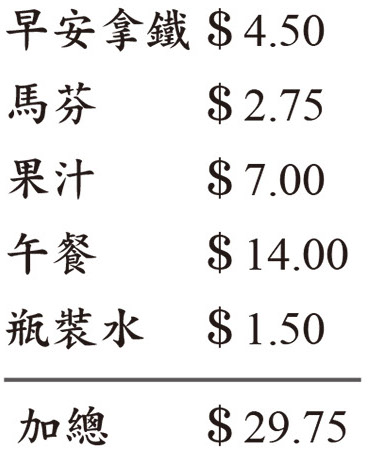
\includegraphics[width=0.25\linewidth]{images/B-136.jpg}
\end{figure}

“还记得我们说的第一条吗，就是第一个小时的薪水先付给自己。”亨利说。“那个退休之后可以变成300万的养老金，每天该存多少啊？”

“25美元。”柔伊嘀咕一声。

亨利点头。“哇，你已经超过了喔！我们还没加上你下午的低咖啡因拿铁。”亨利朝柔伊面前的咖啡点头。“你知道吗，那是可以买下米克诺斯岛泊船照片的。”

她瞪着餐巾纸。

亨利拿起纸巾，递到柔伊面前。

“你的拿铁因子。”他说，“有些也是应该要花的钱。因为，你总要先吃饱。不过，就算午餐必须买，但是不是可以在家煮咖啡，带一盒水果出门？你自己安排一下，每天可以有一半的开支进入退休帐户，这个简单的习惯能给你日后的财务带来大改变。”

她的这番话让柔伊想起刚刚芭芭拉的一番话。

{\kaishu 财务问题的方案是养成新习惯，}

{\kaishu 而不是去赚更多钱。}

柔伊接过了这张纸巾，放入口袋。“所以，我应该做的是记录每一笔小开支，晚上仔细检查，看看有没有可能省下来？”对柔伊来说，这真是最痛苦的折磨。

“不、不、不。”亨利说，“完全不是这个意思。刚好相反，就是不要去记得每一块钱用在哪里。记得我们刚刚说的吗？预算是没用的。我们这样练习只是让你明白，你赚的已经够累积一笔财富了。”

柔伊看着亨利。

“你的意思是说，我比想像的有钱。”柔伊说。

“是的。你比想像的有钱。”亨利重复说。“也就是说，你赚得够多了，足够在财务自由了。就像许多人一样，你的问题在于赚了钱很快就花光。就在放热水洗澡时，同时把排水管打开，却抱怨怎么无法把热水存起来。\textbf{我们把未来的财富都花在一些无关重要的小东西上，甚至在花钱时想都不想}。完全可以在家煮咖啡，却要去咖啡厅买；每天午餐都外食、买瓶装水；订阅付费电视节目，却没空看；新衣服挂满衣柜，许多甚至没穿过。这些都是可以省下的钱。”

“这不是要你别对自己好。而是要改变一点点生活小习惯，改变一点就好。”

“而这一点改变却会改变你的命运。”

当天晚上，柔伊吃了路易吉家的外送披萨和希腊沙拉后，站在厨房看着咖啡机，那还是她去年的生日礼物，从来还没用过。是不是该来用一用？对不对？

或许可以在上班时喝咖啡？公司的咖啡机可以提供许多不同口味。没理由不这么做啊！

然后，是午餐？柔伊想起了芭芭拉的餐盒，不由得叹气。带个午餐去工作，似乎也没那么恐怖。她至少可以做花生酱或果酱三明治。

“哇！哈！”柔伊在小公寓里感慨着。

她环视小公寓，她和室友花了多少钱订阅这些根本没空看的节目？衣橱里有多少她很少穿的新衣服？还有许多其他没有用到的零碎小物？这些东西都显示在她的信用卡帐单上，都显示在循环利息上。如果少了这些，她可以按期缴交信用卡费，那该是怎样的生活？

柔伊叹气。她简直不知道该如何计算每样的花费。她仰头，对着天花板大声说：“有没有人可以帮帮我？”说完，她忍不住笑了，这不就是第三个金钱迷思吗？

柔伊从口袋里掏出那张餐巾纸，在一个桌角摊平看着下方的总和数字：

＄29.75

……她忍不住好奇，这不到30美元到底能做点什么？

柔伊从包里拿出笔电，放到流理台上打开。她在在线找到一个计算复利的网站，将流每日花费四舍五入，以30美元计算，1周5天乘以1年52周，加到税前帐户里，以10％年利率乘以40年 ，最后按下计算键。

她身体往椅背上靠，愣在那里。

她反复输入了3次，得到了下面的数字：

4,110,652

超过400万美元。

“不可能的。”她嘀咕着。怎么可能呢！

她脑中响起了杰弗瑞的声音：去哪里赚10％利息？这点亨利已经解释过了。但是，但是，假如杰弗瑞是对的呢？

她重新输入了数字。这回把利息降到了7％。

1,706,129

如果这样也太乐观了，她这回输入的利息是5％。

991, 913

柔伊瞪着屏幕，简直不敢相信自己的眼睛。即便是以5％计算，也会有近百万的收获。

她关上电脑，想像着自己每天一早处理食材带便当的情景，和在33楼煮咖啡的情景。她真的可以把省下来的拿铁钱和午餐钱放到退休帐户，为她的老年提供优渥的资金吗？

柔伊摇了摇头，好像要把不真实的想法，摇出脑外。

她想起了老妈的笑声，以及老妈说的话：我甚至不会做糖霜。她在电话那头说：柔伊，要为拥有的而开心。

柔伊把笔电放到置于地板的背包里。

她忍不住把和亨利的对话当作一则杂志专文来重新思考。想着这个对话的图片呈现和叙事曲线。她叹气，这不就像是另一篇她要经手的文章吗？别人的想法，别人的冒险旅程，以及别人的成长历程。

这是别人的人生，不是她的。

她手机有短信进来的声音，是洁西卡。

{\kaishu 我们明天下午4:00见？}

明天就是周五了，是回复新工作的最后期限。和洁西卡喝一杯，为新工作干杯。

她还没回信，第二封短信又进来了。

{\kaishu 对了，你和经纪公司谈过了吗？告诉我，你已经搞定了新工作。:-) :-)}

柔伊看着手机屏幕好长时间，才拿起来回复：

{\kaishu 明天下午4:00见。:-)}

柔伊放下手机，起身去刷牙，准备就寝。她躺在床上，瞪着天花板。

她没有心情愉悦到脸上真的绽放笑容。

真的没有，她一点都没有开心的感觉。她也不知道为什么，但此时此刻，她很显然觉得不开心。
